\section{Method}
\label{sec:method}

\begin{figure}[t]
  \centering
  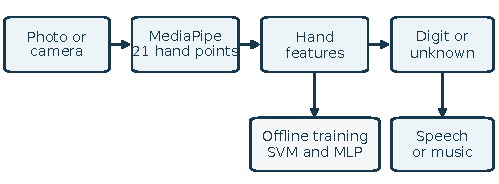
\includegraphics[width=\columnwidth]{pipeline.pdf}
  \caption{The static pipeline. Offline training compares three feature
  sets with two classifiers. At run time the browser applies the exported
  MLP and confirms a stable prediction before triggering output.}
  \label{fig:pipeline}
\end{figure}

\subsection{Data and landmark extraction}

The image collection combines a locally relabeled subset of the Sign Language
Digits Dataset~\cite{mavi2020digits} with additional team photographs for the
digits 6, 7 and 9. Two hand-shape variants are mapped to the label 3 and two
off-vocabulary pose folders are mapped to \texttt{unknown}. The latter class
represents those two pose families. The new photographs were cropped and
resized to $100\times100$ pixels. The 18 new source photographs have 10
derivatives each, generated with rotations, brightness and contrast changes,
scaling, and translations.

We run the MediaPipe Hand Landmarker in image mode for offline images and in
video mode for the webcam. The detector is configured to report up to two
hands. The feature stage requires exactly one detected hand and 21 valid
three-dimensional world landmarks. We log extraction failures before
classification. MediaPipe weights remain frozen in all experiments.

\subsection{Hand representation}

Let $\mathbf{p}_j$ denote the 3-D landmark with index $j$. We translate the
wrist to the origin and scale by the distance from the wrist to the base of
the middle finger:
\begin{equation}
  \mathbf{q}_j =
  \frac{\mathbf{p}_j-\mathbf{p}_0}{\lVert\mathbf{p}_9-\mathbf{p}_0\rVert_2}.
  \label{eq:norm}
\end{equation}
We reflect the horizontal coordinate of a left hand to use a common
handedness convention. Orientation relative to the camera is preserved so
that different palm directions can contribute to classification.

The coordinate representation flattens the 21 normalized points into a
63-element vector. The geometry representation contains ten finger bend
angles (two per finger), three angles between adjacent fingers, four
distances from the thumb tip to the other fingertips, and the three
components of a unit palm normal. We obtain the normal from the cross
product of the wrist-to-index-base and wrist-to-little-finger-base vectors.
Angles are divided by $\pi$. Concatenating both representations yields 83
features.

\subsection{Classification and webcam output}

We compare a support vector classifier with a radial basis kernel ($C=1$)
and a ReLU multilayer perceptron (MLP) with 64 and 32 hidden units, using
scikit-learn~\cite{pedregosa2011sklearn}. The MLP uses Adam and at most 500
training iterations. Each pipeline fits a standard scaler using the training
split only. The resulting scaler and MLP weights are exported for direct
browser inference, as shown in Fig.~\ref{fig:pipeline}.

The speech mode confirms a digit after the predicted class stays stable for
600 ms with a probability of at least 0.8. It latches the prediction to avoid
repeating the same output while the hand is held in place. The application
offers Cantonese, English, and Mandarin audio. The instrument mode uses a
shorter 220 ms confirmation window and maps digit labels to pitches. It
synthesizes piano, guitar, and flute timbres via Web Audio. The audio settings
do not enter the model's feature calculation.
